%(BEGIN_QUESTION)
% Copyright 2009, Tony R. Kuphaldt, released under the Creative Commons Attribution License (v 1.0)
% This means you may do almost anything with this work of mine, so long as you give me proper credit

Undersøk denne delen av et P\&ID. Dette spesifikke diagrammet viser noe av røropplegget og instrumenteringen knyttet til en kjemisk reaktortank:

$$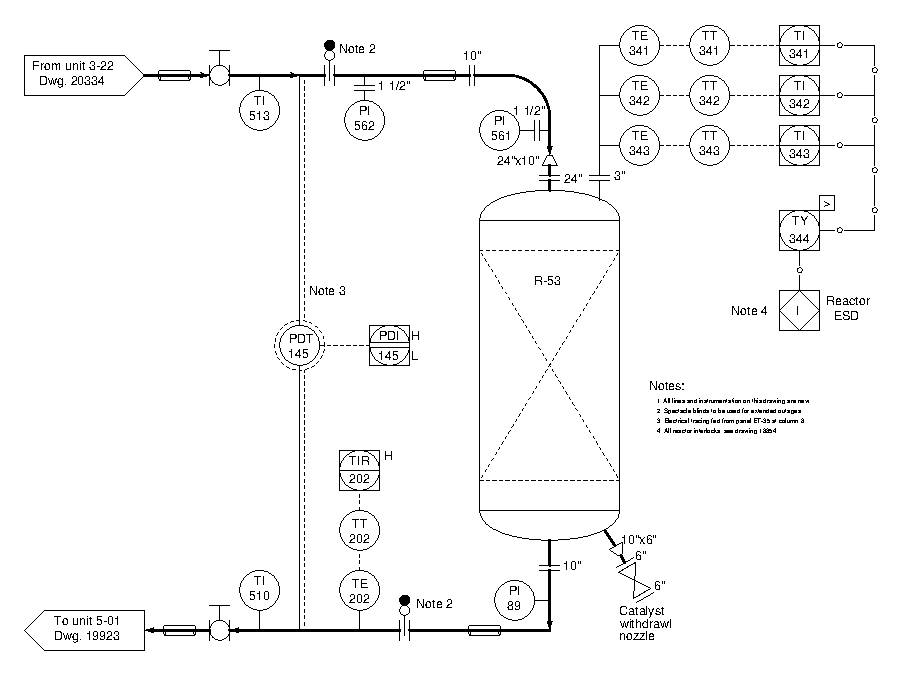
\includegraphics[width=15.5cm]{i03890x01.eps}$$


\begin{itemize}
\item{} Hvilken retning strømmer prosessvæsken gjennom denne reaktortanken? Hvordan kan vi se det ut fra diagrammet?
\vskip 10pt
\item{} Identifiser funksjonene til alle instrumentsymbolene som vises i dette diagrammet, samt betydningen av deres identifikasjonsbokstaver (f.eks. ``PDT'').
\vskip 10pt
\item{} Hvordan vises rør-{\it flenser} i et PFD eller P\&ID?
\vskip 10pt
\item{} Hva er betydningen av de trapesformede symbolene med to størrelser (f.eks. 10" $\times$ 24")?
\vskip 10pt
\item{} To steder i dette diagrammet vises plasseringen av en {\it blindflens} (blind), som brukes til å stenge et rør sikkert ved en flens for vedlikeholdsformål. Finn disse to blindflens-installasjonene i diagrammet.
\vskip 10pt
\item{} Noen av symbolene som vises i dette P\&ID-et fungerer også som prosessalarmer. Identifiser hvilke av indikatorene som også har alarmfunksjoner, og hvilke av disse som er høy-alarmer, lav-alarmer eller begge deler.
\end{itemize}

%\vskip 20pt \vbox{\hrule \hbox{\strut \vrule{} {\bf Forslag til sokratisk diskusjon} \vrule} \hrule}
%
%\begin{itemize}
%\item{} Basert på det du ser i dette P\&ID-et, hva tror du formålet med PDT-145 er?
%\item{} Basert på det du ser i dette P\&ID-et, hva tror du er formålet med å ha {\it tre} temperaturtransmittere på toppen av tanken?
%\item{} Hvordan kryssrefereres ytterligere dokumenter i dette P\&ID-et?
%\item{} Er det avsnitt i læreboken din som kan være til hjelp for å forstå dette P\&ID-et, som ikke eksplisitt ble tildelt som leselekse?
%\end{itemize}
%
\underbar{file i03890no}
%(END_QUESTION)





%(BEGIN_ANSWER)

Hvis en blindflens eller en annen sikkerhetsanordning må forlates i sikker tilstand av en bestemt grunn, må personen som aktiverer sikkerhetsanordningen {\it låse} den på plass og {\it merke} den med et informativt skilt som angir årsaken og varigheten av utkoplingen. Dette kalles vanligvis en {\it lock-out}, {\it tag-out}-prosedyre (LOTO).

%(END_ANSWER)





%(BEGIN_NOTES)

Prosessflyten er fra topp til bunn (følg pilene).

\vskip 10pt

PDT = Differansetrykk-transmitter (Differential pressure transmitter)

TE = Temperaturelement / føler (Temperature element)

PI = Trykkindikator (Pressure indicator)

TY = Temperatur-relé / omformer / beregningsfunksjon (Temperature relay/converter)

\vskip 10pt

Rørflenser vises som korte parallelle linjer vinkelrett på røret.

\vskip 10pt

Trapes = rørovergang (redusering/utvidelse), med rørdimensjoner spesifisert.

\vskip 10pt

Blindflenser har ``Note 2'' ved siden av seg.

\vskip 10pt

Prosessalarmer indikeres med bokstavene ``H'' (høy) og ``L'' (lav) skrevet ved siden av instrumentsymbolene (boblene).

\vskip 10pt














\vskip 20pt \vbox{\hrule \hbox{\strut \vrule{} {\bf Virtuell feilsøking} \vrule} \hrule}

Dette spørsmålet er en god kandidat for en øvelse i ``Virtuell feilsøking''. Når du presenterer diagrammet for studentene, ser du først for deg en bestemt feil i systemet. Deretter presenterer du ett eller flere symptomer på den feilen (noe som kan merkes av en operatør eller annen bruker av systemet). Studentene foreslår så ulike diagnostiske tester som kan utføres på systemet for å identifisere feilens art og plassering, som om de var teknikere som prøvde å feilsøke problemet. Din jobb er å fortelle dem hva resultatet/resultatene ville bli for hver av de foreslåtte testene, og dokumentere disse resultatene slik at alle studentene kan se dem.

Under og etter øvelsen er det lurt å stille studentene oppfølgingsspørsmål som:

\begin{itemize}
\item{} Hva forteller resultatet av den siste diagnostiske testen deg om feilen?
\item{} Anta at resultatene av den siste testen var annerledes. Hva ville det resultatet da fortalt deg om feilen?
\item{} Er den siste diagnostiske testen den beste vi kunne gjort?
\item{} Hva ville være den ideelle rekkefølgen av tester for å diagnostisere problemet i så få trinn som mulig?
\end{itemize}


%INDEX% Process: chemical reactor (realistic P&ID shown)

%(END_NOTES)
